% This is samplepaper.tex, a sample chapter demonstrating the
% LLNCS macro package for Springer Computer Science proceedings;
% Version 2.20 of 2017/10/04
%
\documentclass[runningheads]{llncs}

\usepackage{graphicx}
\usepackage{ae,aecompl}
\usepackage[utf8]{inputenc}
\usepackage[english]{babel}
\usepackage{verbatim}
\usepackage{graphicx}
\usepackage{amsfonts}
\usepackage{amsmath}
\usepackage{amssymb}
\usepackage{stmaryrd}
\usepackage{amstext}
\usepackage{bm} 
\let\proof\relax
\let\endproof\relax
\usepackage{amsthm}
\usepackage{siunitx}
\usepackage{mathrsfs}
\usepackage{wrapfig}
\usepackage{minted}
\usepackage{algorithm}
\usepackage{algpseudocode}
\usepackage{semantic}
\usepackage[dvipsnames]{xcolor}
\usepackage{paralist}
\usepackage{cite}
\usepackage{url}
\usepackage{todonotes}
% Used for displaying a sample figure. If possible, figure files should
% be included in EPS format.
%
% If you use the hyperref package, please uncomment the following line
% to display URLs in blue roman font according to Springer's eBook style:
% \renewcommand\UrlFont{\color{blue}\rmfamily}
% Comments

% Paper specific notation

\setlength{\intextsep}{10pt}

\newcommand{\load}{\ensuremath{\mathit{load}}}
\newcommand{\env}{\ensuremath{\mathit{env}}}
\newcommand{\psu}{\ensuremath{\mathit{psu}}}
\newcommand{\plant}{\ensuremath{\mathit{plant}}}
\newcommand{\ctrl}{\ensuremath{\mathit{ctrl}}}
\newcommand{\fref}{\ensuremath{\mathit{ref}}}
\newcommand{\xaft}{\ensuremath{\mathit{xaft}}}

\newcommand{\inputV}{v}
\newcommand{\consistent}{\ensuremath{\mathit{Consistent}}}
\newcommand{\remaining}{\ensuremath{\mathit{Remaining}}}
\newcommand{\dontcare}{\_}
\newcommand{\defined}{\ensuremath{\mathit{defined}}}
\newcommand{\undefined}{\ensuremath{\mathit{undefined}}}
\newcommand{\properties}{P}
\newcommand{\satisfies}{\vDash}
\newcommand{\simulator}{\mathcal{A}}
\newcommand{\Induced}[2]{\llbracket #1 \rrbracket_{#2}}
\newcommand{\timebase}{\setreal_{\geq 0}}
\newcommand{\stateset}[1]{S_{#1}}
\newcommand{\runstate}[1]{S^{R}_{#1}}
\newcommand{\state}[1]{s_{#1}}
\newcommand{\inputs}[1]{U_{#1}}
\newcommand{\inputvar}[1]{u_{#1}}
\newcommand{\outputs}[1]{Y_{#1}}
\newcommand{\outputvar}[1]{y_{#1}}
\newcommand{\values}{\mathcal{V}}
\newcommand{\true}{\mathit{true}}
\newcommand{\false}{\mathit{false}}
\newcommand{\feedthrough}[1]{D_{#1}}
\newcommand{\reactivity}[1]{R_{#1}}
%\newcommand{\finit}[1]{\mathtt{init}_{#1}}
\newcommand{\fset}[1]{\mathtt{set}_{#1}}
\newcommand{\fget}[1]{\mathtt{get}_{#1}}
\newcommand{\fdoStep}[1]{\mathtt{doStep}_{#1}}
\newcommand{\timestamp}[1]{\varphi(#1)}
\newcommand{\feedsto}[2]{U_{#1}^{#2}}
\newcommand{\master}{\mathcal{A}}
\newcommand{\alloutputs}{Y}
\newcommand{\allfeedthroughs}{D}
\newcommand{\allcontracts}{\mathcal{C}}
\newcommand{\coupling}{L}
\newcommand{\allinputs}{U}
\newcommand{\fmus}{C}
\newcommand{\sequence}[1]{\pargroup{#1}}
\newcommand{\functioncall}{f}
\newcommand{\initcall}{I}
\newcommand{\allfunctioncalls}{F}
\newcommand{\fmu}[1]{\texttt{#1}}
\newcommand{\signal}[1]{\texttt{#1}}
\newcommand{\before}[2]{\ensuremath{#1 \twoheadrightarrow #2}}
\newcommand{\ibefore}[2]{\ensuremath{#1 \rightarrow #2}}
\newcommand{\after}[1]{{#1}'}
\newcommand{\aftern}[2]{{#1}^{(#2)}}
\newcommand{\stateafter}[2]{\ensuremath{\state{#1}^{(#2)}}}


\newtheorem{procedure}{Procedure}{}
\newtheorem{assumption}{Assumption}{}
%\newtheorem{problem}{Problem}{}

\theoremstyle{definition}
%\newtheorem{definition}{Definition}{}
%\newtheorem{example}{Example}{}
\newtheorem{experiment}{Experiment}{}

%\theoremstyle{remark}
%\newtheorem{remark}{Remark}{}




% Generic stuff

\newcommand{\footurl}[1]{\footnote{\url{#1}}}

% Math
\newcommand{\brackets}[1]{\ensuremath{ \left[ #1 \right] }}
\newcommand{\tuple}[1]{\ensuremath{ \left\langle #1 \right\rangle }}
\newcommand{\set}[1]{\ensuremath{ \left\{ #1 \right\}}}
\newcommand{\system}[1]{\ensuremath{ \begin{cases} #1 \end{cases}}}
\newcommand{\rightgroup}[1]{\ensuremath{ \left. \begin{matrix} #1 \end{matrix} \right\} } }
\newcommand{\pargroup}[1]{\ensuremath{ \left( #1 \right)}}
\newcommand{\inv}[1]{\ensuremath{\pargroup{ #1 }^{-1}}}
\newcommand{\dert}[1]{\ensuremath{ \dot{#1} }}
\newcommand{\ddert}[1]{\ensuremath{ \ddot{#1} }}
\newcommand{\partialder}[2]{\ensuremath{ \frac{\partial#1}{\partial#2} }}
\newcommand{\setreal}[0]{\ensuremath{\mathbb{R}}}
%\newcommand{\setbool}[0]{\ensuremath{\mathit{Bool}}}
\newcommand{\setnat}[0]{\ensuremath{\mathbb{N}}}
\newcommand{\norm}[1]{\left\lVert#1\right\rVert}
\newcommand{\bnorm}[1]{\big\lVert#1\big\rVert}
\newcommand{\abs}[1]{\left|#1\right\|}
\newcommand{\xs}[2]{\ensuremath{#1^{\left[#2\right]}}}
\newcommand{\infinitynorm}[1]{\left\lVert#1\right\rVert_\infty}
\newcommand{\bigO}[1]{\ensuremath{ \mathcal{O}\left( #1 \right)}}
\newcommand{\vectorOne}[1]{\brackets{%
\begin{matrix}
  #1
 \end{matrix}%
}}
\newcommand{\vectorTwo}[2]{\brackets{%
\begin{matrix}
  #1 \\
  #2
 \end{matrix}%
}}
\newcommand{\vectorThree}[3]{\brackets{%
\begin{matrix}
  #1 \\
  #2 \\
  #3
 \end{matrix}%
}}
\newcommand{\vectorFour}[4]{\brackets{%
\begin{matrix}
  #1 \\
  #2 \\
  #3 \\
  #4
 \end{matrix}%
}}
\newcommand{\vectorFive}[5]{\brackets{%
\begin{matrix}
  #1 \\
  #2 \\
  #3 \\
  #4 \\
  #5
 \end{matrix}%
}}
\newcommand{\vectorSix}[6]{\brackets{%
\begin{matrix}
  #1 \\
  #2 \\
  #3 \\
  #4 \\
  #5 \\
  #6
 \end{matrix}%
}}
\newcommand{\vectorSeven}[7]{\brackets{%
\begin{matrix}
  #1 \\
  #2 \\
  #3 \\
  #4 \\
  #5 \\
  #6 \\
  #7
 \end{matrix}%
}}
\newcommand{\vectorEight}[8]{\brackets{%
\begin{matrix}
  #1 \\
  #2 \\
  #3 \\
  #4 \\
  #5 \\
  #6 \\
  #7 \\
  #8
 \end{matrix}%
}}

\newenvironment{aligneq*}%
{
\begin{equation*}
\begin{aligned}
}{
\end{aligned}
\end{equation*}
}

\newenvironment{aligneq}%
{
\begin{equation}
\begin{aligned}
}{
\end{aligned}
\end{equation}
}


\begin{document}
%
\title{An FMI-Based Initialization Plugin for INTO-CPS Maestro 2}
%
%\titlerunning{Abbreviated paper title}
% If the paper title is too long for the running head, you can set
% an abbreviated paper title here
%
\author{Simon Thrane Hansen\inst{1} \and
Casper Thule\inst{1}}
%
\authorrunning{S. Thrane and C. Thule}
% First names are abbreviated in the running head.
% If there are more than two authors, 'et al.' is used.
%
\institute{DIGIT, Department of Engineering, Aarhus University, \email{\{sth, casper.thule\}@eng.au.dk\}}}
%
\maketitle              % typeset the header of the contribution
%

\begin{abstract}
The development of cyber-physical systems (CPS) is challenging due to the heterogeneity of the different subsystems. To assist in the development process, co-simulation can be used, where models of constituents of a CPS are coupled to jointly simulate the behavior of the full system. However, a trustworthy result of the co-simulation is only obtained if all of the simulation units are initialized correctly and in the correct order. In this work, we consider co-simulation where the simulation units are described as Functional Mock-up Units (FMU). The Functional Mock-up Interface specification specifies constraints to the initialization of variables in the scope of a single FMU. However, it does not consider the initialization of interconnected variables between instances of FMUs. Such interconnected variables place particular constraints on the initialization order of the FMUs.\\
The approach taken to calculate a correct initialization order is based on predicates from the specification and the topological ordering of both internal connections and interconnected variables. Circular dependencies between FMU variables are dismissed. %This approach has been compared to other already existing approaches for FMI initialization. 
The approach has been realized as a plugin for the open-source INTO-CPS Maestro 2 Co-simulation framework. It has been tested for various scenarios and compared to an existing \textit{Initializer} that has been validated through academic and industrial application.

\keywords{Co-simulation \and Initialization \and Topological ordering \and FMI}
\end{abstract}

%The correct initialization of a co-simulation depends not only on the value being assigned to each port but also the order in which the ports are initialized.





\section{Introduction}\label{sc:introduction}
Cyber-physical systems (CPS) are becoming ever more sophisticated, while market pressure shortens the available development time. One of the tools used to manage the increasing complexity of such systems is co-simulation since it addresses their various parts of heterogeneous nature. Co-simulation is a technique to combine multiple black-box simulation units to simulate/compute the behavior of the combined models as a discrete trace\cite{Kubler2000}. \\
The Functional Mock-up Interface (FMI) standard \cite{Blochwitz2012, fmi_2019} prescribes an interface for how to communicate with each simulation unit. This interface can be used to connect different simulation units (called Functional Mock-up Units or FMUs) and exchange values between them and make them progress in time. \\
A typical co-simulation consists of three phases: Initialization, simulation, and teardown. This work concentrates on the first of these phases - the initialization phase. FMI specifies criteria for how an FMU shall be initialized. However, the FMI standard is not concerned with how a connected system of multiple FMUs should be correctly initialized as a whole. 
The way a system of multiple FMUs should be initialized and interacted with depends on each FMUs implementation and interconnections to other FMUs \cite{gomes_lucio_vangheluwe_2019}, since these place precedence constraints between the FMU variables. The precedence constraints make specific system configurations and initialization orders of a system invalid due to cyclic dependencies and dependencies among the interconnected variables. An appropriate order of initialization is vital for the correctness of the co-simulation \cite{Thule2018} because it ensures a variable is never read before it is set.\\
This paper describes an approach for the initialization of an FMI-based co-simulation. The approach complies with the semantics of FMI and ensures the absence of cycles in the system. The approach does not put any constraints on choosing a master algorithm that should be used to carry out the simulation. This means that the approach is suitable to combine with well-established master algorithms like Gauss-Seidel and Jacobian \cite{Palensky2017}. The approach has been realized as a plugin to the co-simulation framework called INTO-CPS Maestro 2 (Maestro 2). The realized plugin has been tested for various scenarios and compared to an existing \textit{Initializer} that has been validated through academic and industrial applications.

\noindent Structure: Section \ref{sc:background} gives a brief background of the formalization of FMUs and Maestro 2. Section \ref{sc:initilization} describes the approach taken to calculate the initialization order. This is followed by section \ref{sc:implementation}, where the realization of the approach is presented. Finally, section \ref{sc:summary} provides concluding remarks and describes future work.


\section{Background}\label{sc:background}
In this section, we provide a formalization of FMI co-simulation and a short background on Maestro 2.

\subsection{FMU definitions}
To describe the formalization of FMUs the vocabulary is adopted by Gomes et al\cite{gomes_lucio_vangheluwe_2019, Gomes2018}. The main definitions of relevance to this paper will be presented, but for more information readers are referred to the original publications. 
\begin{definition}[FMU]\label{def:fmu}
  An FMU with identifier $c$ is represented by the tuple   
  $$\tuple{\stateset{c}, \inputs{c}, \outputs{c}, \fset{c}, \fget{c}},$$
  where:
  \begin{inparadesc}
    \item $\stateset{c}$ represents the state space;
    \item $\inputs{c}$ and $\outputs{c}$ the set of input and output variables, respectively;
    \item $\fset{c} : \stateset{c} \times \inputs{c} \times \values \to \stateset{c}$ and $\fget{c}: \stateset{c} \times \outputs{c} \to \values$ are functions to set the inputs and get the outputs, respectively (we abstract the set of values that each input/output variable can take as $\values$).
  \end{inparadesc}
\end{definition}

\begin{definition}[Scenario]\label{def:cosim_scenario}
  A scenario is a structure $\tuple{\fmus, \coupling}$ where each identifier $c \in \fmus$ is associated with an FMU, as defined in \ref{def:fmu}, and $\coupling(u)=y$ means that the output $y$ is connected to input $u$.
  Let $\allinputs = \bigcup_{c \in \fmus} \inputs{c}$ and $\alloutputs = \bigcup_{c \in \fmus} \outputs{c}$, then $\coupling : \allinputs \to \alloutputs$.
\end{definition}

\begin{definition}[Feed-through]\label{def:feedthrough}
  The input $\inputvar{c} \in \inputs{c}$ feeds through to output $\outputvar{c} \in \outputs{c}$, that is, $(\inputvar{c},\outputvar{c}) \in \feedthrough{c}$, when there exists $v_1, v_2 \in \values$ and $\state{c} \in \stateset{c}$, such that
  $
  \fget{c} (\fset{c}(\state{c}, \inputvar{c}, v_1), \outputvar{c}) \neq \fget{c} (\fset{c}(\state{c}, \inputvar{c}, v_2), \outputvar{c}).
  $
\end{definition}

\begin{definition}[Output Computation]\label{def:getout}
The $\fget{c}(\dontcare, \outputvar{c})$ represents the calculation of output $\outputvar{c}$ of $c \in \fmus$. Given a co-simulation state, it checks whether all inputs that feed-through to $\outputvar{c}$ are defined.
\end{definition}

\begin{definition}[Input Computation]\label{def:setin}
The $\fset{c}(\dontcare, \inputvar{c}, \inputV)$ represents the setting of input $\inputvar{c}$  of $c \in \fmus$. Given a co-simulation state, it checks whether all outputs connected to I are defined.
\end{definition}

\subsection{INTO-CPS Maestro 2}
INTO-CPS Maestro 2\footnote{currently in alpha \url{https://github.com/INTO-CPS-Association/maestro/tree/2.0.0-alpha}}\cite{thule_maestro2_2019} is an FMI-based co-simulation framework set to supersede Maestro\cite{Maestro}. The philosophy of the framework is to apply plugins to generate co-simulation specifications expressed in the domain specific language called Maestro Base Language (MaBL). Such specifications are then interpreted and executed resolving in the execution of a co-simulation.

\section{Generation of an Initialization Order}\label{sc:initilization}
FMI defines certain information about the initialization order described through different states of a co-simulation. The initialization phase covers the two states (in chronological order): \textit{Instantiated} and \textit{Initialization Mode}.
In each of the two states, different groups of FMU variables can be assigned a value. The groups are defined by FMI based on predicates on the characteristics of the variables (\textit{causality}, \textit{initial} and \textit{variability}). These predicates have been extracted and used in the implementation. 
An example of a group is the \textit{INI}-group that consists of FMU variables with $initial = exact\, \lor initial = \,approx $  and $variability \neq constant$. All variables of this group should be set in the \textit{Instantiated}-phase of a co-simulation, and since they have no dependencies/connections to other FMU variables, the order is insignificant. 

In the \textit{Initialization Mode} state, the variables of all FMUs should be defined if no circular dependencies exist. 
The variables with \textit{causality = parameter} of each FMU are set first, and the order of which they are set is again insignificant as they are independent.
Afterwards the interconnected variables should be defined, but as stated by the definitions \ref{def:feedthrough}, \ref{def:getout} and \ref{def:setin} the operations \textit{get} and \textit{set} \textbf{require} a specific initialization order. 

The correct initialization order of these interconnected variables has been calculated using the method described in Gomes et al.\cite{Gomes2019b}. The method is to use a topological ordering as the initialization order. The topological ordering is based on a graph of the interconnected FMU variables and internal connections. The correctness of this approach of using the topological order as the initialization order is justified by a sketch proof and the verification of the algorithm in \textit{prolog} by Gomes et al.
The calculation of the initialization order is linear in the number of both external and internal interconnections. The calculation should also identify circular dependencies between the interconnected FMU variables, since they would invalidate the result of the co-simulation.


\subsection{Structure of the graph}
The graph is constructed based on the interconnected variables and internal connections. Each interconnected variable in the system represents a node, and the edges are based on these connections. The edges of this graph represent precedence constraints based on the algebraic dependencies of the interconnected variables. 

\begin{definition}[Initialization Graph]\label{def:initialization_graph}
  Given a co-simulation scenario $\tuple{\fmus, \coupling}$, and a set of feed-through dependencies $\bigcup_{c \in \fmus} \set{\feedthrough{c}}$, we define the initialization graph where each node represents a port $\outputvar{c} \in \outputs{c}$ or $\inputvar{c} \in \inputs{c}$ of some fmu $c \in \fmus$. The edges are created according to the following rules:
  \begin{compactenum}
    \item For each $c \in \fmus$ and $\inputvar{c} \in \inputs{c}$, if $\coupling(\inputvar{c}) = \outputvar{d}$, add an edge $\outputvar{d} -> \inputvar{c}$.
    \item For each $c \in \fmus$ and $(\inputvar{c},\outputvar{c}) \in \feedthrough{c}$, add an edge $\inputvar{c} -> \outputvar{c}$.
  \end{compactenum}
\end{definition}

\subsection{Single water tank example}
The structure of the Initialization graph will be described using a small example. This is based on a single water-tank where the water level of the tank is controlled by a discrete-event controller. When the water level of the tank reaches a particular level (defined in the controller) the controller sends a command to the tank to empty using an exit valve. An illustration and a diagram of the interconnections of the ports in the system can be in figure \ref{fig:watertank}.

\begin{figure}[H]
    \centering
    \begin{minipage}{0.35\textwidth}
        \centering
    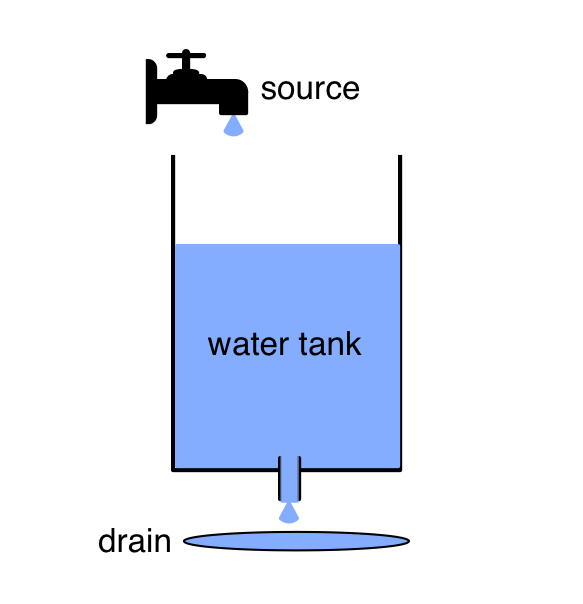
\includegraphics[width=1\textwidth]{images/singletank.png}
    \end{minipage}\hfill
    \begin{minipage}{0.55\textwidth}
        \centering
    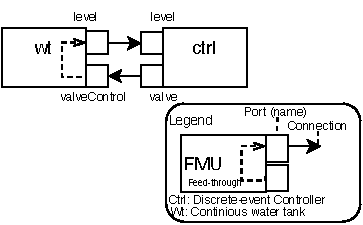
\includegraphics[width=1\textwidth]{images/waterTankFMU-Page-1.pdf}
    \end{minipage}
    \caption{Single water-tank case study}
    \label{fig:watertank}
\end{figure}


\begin{wrapfigure}[6]{r}{0.4\textwidth}
  \begin{center}
  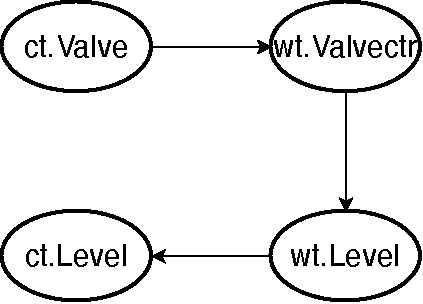
\includegraphics[width=0.30\textwidth]{images/InitializationGraph.pdf}
  \end{center}
    \caption{Initialization graph of water-tank}
  \label{fig:initilizationGraph}
\end{wrapfigure}
\noindent A correct initialization order can be calculated since there is no circular dependencies. The initialization graph of the system can be seen in figure \ref{fig:initilizationGraph}. The correct order of initialization can easily be seen from the figure. But this approach also scales.% to more advanced examples like the Line Follower Robot \footnote{\url{https://github.com/INTO-CPS-Association/example-line_follower_robot}}.
%However, knowledge about the internals of the system is needed in order to calculate this because if we treated the system as a black-box, we would not have taken the internal connection of \textit{WT} into account. An incorrect initialization order could, therefore, have been derived without some knowledge about the feed-through dependencies in the system.  
\newline
\newline
\newline
\newline
\section{Realization of a Maestro 2 Plugin}\label{sc:implementation}
This approach has been realized as a Maestro 2 plugin that generates the \textit{Initialization}-phase of a co-simulation specification expressed in MaBL. It calculates the specification on a list of FMU-components, information of the simulation environment, and specific plugin-configurations describing the connections between interconnected variables. The plugin uses a optimization to group operations that can be executed in parallel to take advantage of FMI's ability to set/get multiple variables in bulk.
The developed plugin has been tested on numerous co-simulation examples and checked against the existing \textit{Initializer} of Maestro.

The topological sorting algorithm was implemented in Scala. The choice of Scala is motivated by the relation to JVM and the connection to Slang and the Logika framework\cite{inbook}. The connection to Slang and Logika will be used in the future work of formally verifying the plugin.

The algorithm for calculating the topological order of the Initialization graph defined in definition \ref{def:initialization_graph} was Tarjan's algorithm. The algorithm was chosen because it solves two of the central issues of the initialization of a co-simulation - identifying circular dependencies (strongly connected components) and performing a topological sorting \cite{tarjan_1972}. The algorithm is furthermore well-established, and there exist formal proofs of its correctness and properties\cite{stefan_merz}. 


\section{Concluding remarks}\label{sc:summary}
This work used a topological ordering based on the interconnected FMUs variable and internal FMU connections along with predicated from the FMI specification to calculate a correct initialization order for a co-simulation. This approach can be combined with an arbitrary master algorithm. 
The approach was realized as a plugin for the open-source INTO-CPS Maestro 2 tool and verified against the existing \textit{Initializer}.
Future work includes formally verifying the plugin, and its implementation of the algorithm used to calculate the topological ordering using the Logika framework.

\paragraph*{\textbf{Acknowlegements.}}We would like to thank Stefan Hallerstede, Peter Gorm Larsen and Claudio Gomes for providing valuable input to this paper and the developed plugin.
%
% ---- Bibliography ---

\bibliographystyle{splncs04}
\bibliography{gen_bib}


\end{document}
